\documentclass[twoside,twocolumn, 12pt]{paper}

%% Escrevendo em português:
\usepackage[brazil]{babel}
\usepackage[utf8]{inputenc}
\usepackage[pdftex]{hyperref}
\usepackage{epstopdf}
\usepackage{psfrag}
\usepackage{setspace}
\usepackage{graphicx}
\usepackage{color}
\usepackage[hang, small,labelfont=bf,up,textfont=it,up]{caption}
\usepackage{subcaption}
\usepackage{float}
\usepackage{amsmath}
\usepackage{amsfonts}
\usepackage{amssymb}
\usepackage{grafcet}
\usepackage{pdfpages}

\usepackage{enumitem} % Customized lists
\setlist[itemize]{noitemsep} % Make itemize lists more compact
%----------------------------


\newtheorem{teorema}{Teorema}%[chapter]
\newtheorem{problema}[teorema]{Problema}
\newtheorem{conj}[teorema]{Conjectura}
\newtheorem{lema}[teorema]{Lema}
\newtheorem{exerc}[teorema]{Exercício}

\definecolor{lightgray}{gray}{0.95}

% Ad hoc macros
\newcommand{\qed}       {\hfill\Box}
\newcommand{\card}[1]   {\left|#1\right|}
\newcommand{\nct}       {\chi_{_T}}
\newcommand{\cnk}[2]    {C_{#1}^{#2}}
\newcommand{\ed}[2]     {#1#2}
\newcommand{\teto}[1]   {\lceil #1 \rceil}
\newcommand{\piso}[1]   {\lfloor #1 \rfloor}
\newcommand{\itab}[1]{\hspace{0em}\rlap{#1}}
\newcommand{\tab}[1]{\hspace{.2\textwidth}\rlap{#1}}


\usepackage{titling} % Customizing the title section

\usepackage{hyperref} % For hyperlinks in the PDF
\usepackage{lettrine} % The lettrine is the first enlarged letter at the beginning of the text

\usepackage{abstract} % Allows abstract customization
\renewcommand{\abstractnamefont}{\normalfont\bfseries} % Set the "Abstract" text to bold
\renewcommand{\abstracttextfont}{\normalfont\small\itshape} % Set the abstract itself to small italic text

\usepackage{titlesec} % Allows customization of titles
\renewcommand\thesection{\Roman{section}} % Roman numerals for the sections
\renewcommand\thesubsection{\Alph{subsection}} % roman numerals for subsections
\titleformat{\section}[block]{\large\scshape\centering}{\thesection.}{1em}{} % Change the look of the section titles
\titleformat{\subsection}[block]{\large}{\thesubsection.}{1em}{} % Change the look of the section titles
%----------------------------------------------------------------------------------------
%	TITLE SECTION
%----------------------------------------------------------------------------------------

\setlength{\droptitle}{-4\baselineskip} % Move the title up

\pretitle{\begin{center}\Huge\bfseries} % Article title formatting
	\posttitle{\end{center}} % Article title closing formatting
\title{Automação no Processo de Fabricação de Cerveja\\ 
	\large Etapas de Maturação e Filtração} % Article title
\author{%
	\textsc{Daniel D. R. Oliveira}\\[1ex]
	\normalsize Faculdade de Engenharia Mecânica\\
	\normalsize Universidade Estadual de Campinas\\
	\and
	\textsc{Marcelli Tiemi Kian}\\[1ex]
	\normalsize Faculdade de Engenharia Mecânica\\
	\normalsize Universidade Estadual de Campinas\\
	\and
	\textsc{Vinicius Ragazi David}\\[1ex]
	\normalsize Faculdade de Engenharia Mecânica\\
	\normalsize Universidade Estadual de Campinas\\
}
\date{\today} % Leave empty to omit a date
\renewcommand{\maketitlehookd}{%
	\begin{abstract}
		\noindent Esse artigo trata de uma abordagem para a automação do processo de maturação e filtragem de cerveja. Ele comtempla o aspecto funcional e implementação do problema em CLP e software supervisório.\\
		
		Palavras Chaves: Controle de Temperatura, Acionamento de válvulas, CLP, Software Supervisório, Grafcet
	\end{abstract}
}

%%%%%%%%%%%%%%%%
\begin{document}
	%%%%%%%%%%%%%%%%
	
\begin{titlepage}
\begin{center}	

\newcommand{\HRule}{\rule{\linewidth}{0.5mm}}
% Upper part of the page. The '~' is needed because \\
% only works if a paragraph has started.

\includegraphics[width=0.15\textwidth]{logoUnicamp}~\\[1cm]

\textsc{\LARGE Universidade Estadual de Campinas}\\[1.5cm]

\textsc{\Large Faculdade de Engenharia Mecânica}\\[0.5cm]

% Title
\HRule \\[0.4cm]
{ \Large \bfseries{ES926 - Automação Industrial\\ \vspace{0.8cm} Projeto Final}\\
\large{Maturação no processo de Fabricação de Cerveja}\\[0.4cm] }

\HRule \\[1.5cm]

% Author and supervisor
\begin{minipage}{0.6\textwidth}
\begin{flushleft} \large
\emph{Nome:}\\
Daniel Dello Russo Oliveira\\ Marcelli Tiemi Kian\\ Vinicius Ragazi David
\end{flushleft}
\end{minipage}
\begin{minipage}{0.2\textwidth}
\begin{flushright} \large
\emph{RA}\\ 101918\\
117892\\ 120258
\end{flushright}
\end{minipage}

\vfill

% Bottom of the page
{\large \today}

\end{center}
\end{titlepage}

	\maketitle
	
	%%%%%%%%%%%%%%%%%%%%%%%%%%%%%%%%%%%%%%%%%%
	\section{Descrição do Problema}
	No processo de fabricação da cerveja, logo após a fermentação, é comum deixar que a bebida passe por uma "fermentação secundária" conhecida como maturação. Durante a maturação ocorre a redução na concentração de ácido sulfídrico, de acetaldeído e de diacetil, produtos da fermentação que afetam o sabor da cerveja. Esse processo também é importante pois nele ocorre a clarificação da cerveja através da precipitação das leveduras e de proteínas que dão um aspecto turvo ao produto. É importante controlar a temperatura e o tempo de maturação de maneira a garantir as características desejadas para a cerveja, tipos diferentes de cerveja precisam ser maturadas em temperaturas e por durações diferentes. A clarificação da cerveja pode ser completada com um processo de filtração pós maturação a fim de remover as partículas em suspensão.
	
	\section{Descrição Técnica do Processo}
	
	Este relatório consiste na descrição da solução encontrada para o problema da maturação e filtragem da produção de cerveja. O processo começa após a fermentação da cerveja verde (pós fermentação) que é mandada para tanques de maturação como o da figura \ref{fig:maturador} (válvula $V_{cv}$ e $timer_1$). No tanque a cerveja verde permanece no taque por um tempo variado ($timer2$) com controle constante de sua temperatura, esta necessitando estar em um intervalo específico de temperaturas. Este controle de temperatura será feito com base no acionamento do fluido refrigerante ($V_{fr}$) e em um sensor de temperatura ($S_t$).
	
	\begin{figure}
		\centering
		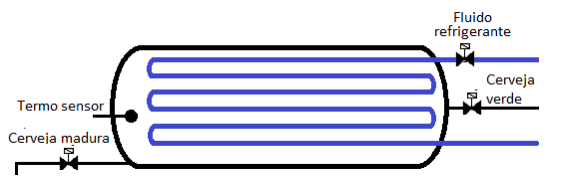
\includegraphics [width=\columnwidth]{tanque.png}
		\caption {Tanque de maturação da cerveja verde.}
		\label{fig:maturador}
	\end{figure}
	
	Passado este tempo e com sucesso do controle de temperatura a cerveja verde torna-se cerveja madura e é despeja na próxima etapa (válvula $V_{cm}$). A etapa consiste em passar por um filtro com terra diatomácea (válvula $V_{td}$), que retira partículas desagradáveis à cerveja, como o mostrado na figura \ref{fig:filtro}. 
	
	O resíduo do filtro deve ser descartado após o uso, o seu descarte é feito pela acionamento de uma válvula ($V_r$) que dependerá de um sensor ($S_{bf}$).
	
	
	Tanto a válvula de despejo da cerveja maturada quanto a da terra diatomácea dependem do sensor de volume do tanque de maturação ($S_{bm}$).
	
	\begin{figure}
		\centering
		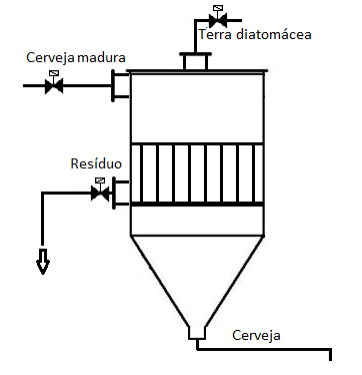
\includegraphics [width=\columnwidth]{filtro.png}
		\caption {Filtro da cerveja maturada}
		\label{fig:filtro}
	\end{figure}
	
	Após a filtragem a cerveja é então destinada à próxima etapa da sua fabricação, sendo esta não descrita por este trabalho.
	
	\section {Análise do Projeto}
	\label{sec:analise}
	Para a primeira etapa do projeto nós acrescentamos um sensor de nível baixo no taque do maturador, afim de verificar que este está de fato vazio antes de preenchê-lo com cerveja verde. Como não existe perigo de que muita cerveja verde seja fornecida para o tanque (uma vez que a quantidade disponível é limitada pelo tamanho do tanque anterior no processo), o procedimento é controlado através de um timer, estimamos que 10 minutos seja tempo mais que suficiente para preencher o tanque. Deixamos então a cerveja maturar por 2 horas, controlando a sua temperatura através de sensores.
	
	Enquanto o  tanque está sendo preenchido e durante o processo de maturação da cerveja, podemos realizar de maneira paralela a liberação dos resíduos do filtro, contanto que não exista mais cerveja maturada para ser filtrada, verificamos isso através de um sensor colocado um pouco abaixo do nível do filtro. Abrimos a válvula para liberação dos resíduos e a deixamos aberta até que a cerveja no maturador acabe de maturar, como a maturação é um processo lento, teremos tempo de sobra para esvaziar o filtro.
	
	Uma vez maturada, a cerveja segue para o a filtração onde receberá terra diatomácea. O controle da proporção entre cerveja e terra diatomácea se dá pela configuração manual das válvulas de liberação de ambas e não será abordada pelo programa.
	
	A figura \ref{fig:grafcet} mostra um diagrama grafcet da nossa implementação do processo.
	
	\begin{figure*}[t]
		\centering
		\begin{tikzpicture}
			\EtapeInit[0,0]{0}
			\Transition[VX0]{0}
			\DivET{T0}{-7.5/L10,7.5/L20}
			\Etape[VL10]{10}
			\Transition[VX10]{10}
			\EtapeEncapsulante[VT10]{20}
			\SequenceEE[VL20]{11}{21}
			\ConvET[7.5]{X20}{X21}{br3}
			\Transition[br3]{br3}
			\Etape[VTbr3]{4}
			\Transition[VX4]{4}
			\LienRetour[10]{T4}{X0}
			\ActionX{X10}{$V_{cv}$, inicia $timer_1$}
			\ActionActiv{X10}
			\ActionX{X20}{inicia $timer_2$}
			\ActionActiv{X20}
			\ActionX{X21}{$V_r$}
			\ActionX{X4}{$V_{cm}$,$V_{td}$}
			\Recept{T0}{$\overline{S_{bm}}\cdot Start$}
			\Recept{T10}{$timer_1 > 10m$}
			\Recept{Tbr3}{$timer_2 > 2h$}
			\Recept{T11}{$\overline{S_{bf}}$}
			\Recept{T4}{$\overline{S_{bm}}$}
			
			\begin{Encap}[nom]{6.0,-1.5}{20}{Refrigeração}
			\Etape[0,0]{200}
			\Transition[VX200]{200}
			\Etape[VT200]{300}
			\Transition[VX300]{300}
			\LienRetour{T300}{X200}
			\LienActivation{X200}
			\ActionX{X300}{$V_r$}
			\Recept{T200}{$S_t \geq 5ºC$}
			\Recept{T300}{$S_t \le -5ºC$}
			\end{Encap}
			
			\draw[red,thick,dashed] (-3.75,-1.75) -- (2,-1.75) -- (2, -5.4) -- (-3.75, -5.4) -- cycle;
			
			\draw[red,thick,dashed] (2.3,-1.75) -- (5.5,-1.75) -- (5.5, -5.4) -- (5.5, -8.7) -- (-1, -8.7) -- (-1, -6) -- (2.3, -6) -- cycle;
		\end{tikzpicture}
		\caption{Diagrama grafcet do projeto}
		\label{fig:grafcet}
	\end{figure*}
	
	\subsection{Modo Automático}
	O modo automático consiste na ciclagem automática entre os estados do sistema. Este é o modo padrão de operação do sistema e não necessita de um funcionário presente para fazer as transições. Quando o sistema está na posição home e no modo automático, este aguarda que seja pressionada a chave Iniciar para começar sua execução. Caso este esteja no modo homming e seja transferido para o automático, ele continuará seu ciclo normalmente até que volte para home e então aguardará o botão Iniciar para entrar no modo automático. A implementação de tal lógica pode ser vista na seção \ref{sec:ladder} nas redes 2 a 4. 
	
	\subsection{Modo Homming}
		
	O modo Homming, ao contrário do modo Automático, faz com o que o sistema pause entre os ciclos de operação. A transição entre a posição ``home" e a próxima somente ocorrerá quando o botão ``Iniciar" da IHM for apertado. Um ciclo de homming só termina quando o sistema atinge sua posição inicial (``home"), sendo que a transição entre o modo Homming e o modo Automático somente será efetuada quando o sistema se encontrar nesta posição. O modo Homming é útil durante a configuração inicial do sistema e a etapa de testes/validação. Sua implementação pode ser vista na seção \ref{sec:ladder} nas redes 2 a 4. 
	
	
	\subsection{Modo Passo a Passo}

	O modo passo a passo facilita a depuração e teste do sistema, introduzindo a necessidade a atuação humana para a transição entre estados. Com todas as condições de transição verificadas o processo apenas mudará de estado caso um botão na IHM (Passo) seja apertado manualmente. Caso as condições de transição não sejam obedecidas e o operador pressionar o botão na IHM nada acontecerá.
	
	Sua utilidade é comprovada durante os testes, já que o processo pode ser totalmente controlado pelo engenheiro de qualidade, testando todas as transições e funcionalidade das entradas (sensores e timers) do sistema. A implementação do modo passo a passo pode ser vista na seção \ref{sec:ladder} nas redes 5 a 9.
	
	\subsection{Parada de emergência}
	Quando o botão de emergência da IHM (interface homem-máquina, figura \ref{fig:ihm}) é ativado, os estados ativos são enviados para seu estado equivalente de emergência, como pode ser visto na implementação na rede 24 da seção \ref{sec:ladder}. Por motivos de segurança, todos os atuadores são desativados (todas as válvulas são fechadas, incluindo a responsável pelo fluido refrigerante que não tem contato direto com o produto), até que o sistema saia do estado de emergência ao desativar o botão da interface gráfica. 
	
	No processo de saída do estado de emergência, conforme a rede 23 da seção \ref{sec:ladder}, cada estágio que estava em modo de emergência é retomado, cabendo ao operador determinar a validade ou não do lote que ficou parado na produção dependendo do tempo em que o sistema ficou em emergência e da circunstância que levou à parada, pois pode ou não afetar a integridade do produto. Esta decisão é de certa maneira delicada, e não foi possível automatizá-la. 
	
	\subsection{Alarmes e tratamentos de Erros}
	%TODO Revisar, principalmente tempos das condições de alarme e o que isto pode significar
	Para a implementação do sistema de alarmes, utilizamos um conjunto de situações que não afetavam de imediato a produção, mas que necessitam de atenção do operador. Estas situações são descritas abaixo, junto com os cuidados que devem ser tomados caso aconteça a situação de alarme. Está implementada nas redes 18 a 22 na seção \ref{sec:ladder}.
	\begin{itemize}
		\item Temperatura da cerveja no maturador ficar menor que $-10^oC$ ou maior que $30^oC$: Indica problemas com sensor de temperatura ou com a válvula de fluido refrigerante, além de indicar que a temperatura saiu do intervalo desejado e que pode ter comprometido o lote de cerveja em produção.
		\item Tempo para atingir o nível baixo do filtro maior que $30$ minutos: Indica problemas com o sensor de nível baixo do filtro ou com sua permeabilidade, que pode causar atrasos na linha de produção.
		\item Tempo de resfriamento da cerveja no maturador maior que $30$ minutos: Indica problemas com o sensor de temperatura ou com o sistema de refrigeração (válvula defeituosa, vazamento no fluido de refrigeração, entre outros), podendo causar distúrbios na temperatura de maturação.
		\item Tempo de saída da cerveja madura maior que $10$ minutos: Indica problemas na válvula de saída ou no sensor de nível baixo do maturador.
	\end{itemize}
	
	Quando o sistema se encontra em situação de alarme, um LED de alarme é aceso na IHM (interface homem-máquina), e só pode ser apagado quando todas as condições de alarme forem resolvidas e o operador pressionar a tecla para desligar o alarme (Reset Alarme) na IHM.
	
	\subsection{IHM}
	%TODO Revisar
	A IHM (Interface Homem-Máquina) do sistema mostrada na figura \ref{fig:ihm} possui entradas e saídas para que o operador consiga controlar o andamento da produção, obtendo dados do que está acontecendo com ela. 
	
	As saídas da IHM são basicamente duas luzes do lado superior esquerdo identificadas com o símbolo *, uma vermelha para identificar uma situação de alarme, e outra verde quando o sistema está em ``Home", e também pode-se acompanhar a variação de temperatura no maturador mostrada no centro da tela identificado também com o símbolo *.
	
	Conforme explicado anteriormente, é possível escolher modos de operação, como o ``Homming" ou ``Automático" pela chave seletora na parte inferior esquerda (identificada pelo número 1), ativar ou desativar a execução ``Passo a passo" pela chave ao lado (identificada pelo número 2).	Para ativar e desativar o modo de emergência pela chave em destaque no lado direito superior.
	
	No modo ``Passo a Passo" após o sistema conseguir as condições para mudar de estado, deve-se pressionar a tecla ``Passo" (identificado por 4) na parte inferior direita da tela para efetuar a transição. No modo ``Homming" é necessário apertar o botão ``Iniciar" na parte superior central (identificado por 5) para começar um novo ciclo quando o sistema se encontra em ``Home". Em caso de estado de alarme, deve-se reparar as condições que causaram o alarme e em seguida apertar o botão ``Reset Alarme" do lado direito no centro (identificado por 6) para desativá-lo.
	
	Os detalhes da implementação da IHM podem ser vistas no apêndice \ref{apx:ihm}.
	
	\begin{figure}
		\centering
		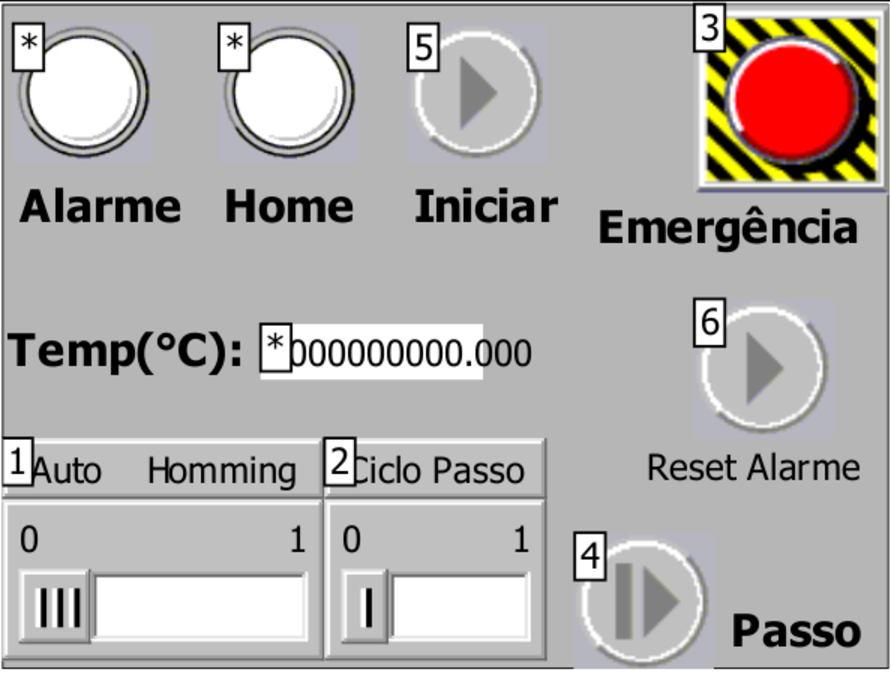
\includegraphics [width=0.8\columnwidth]{ihmsmall.pdf}
		\caption{IHM (Interface Homem-Máquina) do sistema}
		\label{fig:ihm}
	\end{figure}

\section {Tabela de designação}
\begin{table*}[b]
	\caption{Tabela de Entradas}
	\label{tab:in}
	\centering
	\begin{tabular}{|  p{2cm} | p{10cm} | p{2cm} | }
		\hline
		Entrada & Utilidade & Posição\\
		\hline
		$S_{bm}$ & sensor de volume baixo no tanque de maturação & $\%I1.0$ \\
		$S_t$ & sensor de temperatura no tanque de maturação & $\%MD1$ \\
		$S_{bf}$ & sensor de volume baixo do filtro & $\%I1.1$ \\
		\hline
	\end{tabular}
\end{table*}


\begin{table*}[b]
	\caption{Tabela de Saídas}
	\label{tab:out}
	\centering
	\begin{tabular}{|  p{2cm} | p{10cm} | p{2cm} | }
		\hline
		Atuador & Utilidade & Posição\\
		\hline
  		$V_{cv}$ & acionamento da válvula da cerveja verde & $\%Q6.3$ \\
  		$V_{cm}$ & acionamento da válvula da cerveja maturada & $\%Q6.2$ \\
 		$V_{fr}$ & acionamento da válvula de fluido refrigerante & $\%Q7.0$ \\
		$V_{td}$ & acionamento da válvula de terra diatomácea & $\%Q7.1$ \\
		$V_r$ & acionamento da válvula de descarte & $\%Q7.2$ \\
 		\hline
	\end{tabular}
\end{table*}


\begin{table*}[b]
	\caption{Tabela de Temporizadores}
	\label{tab:temp}
	\centering
	\begin{tabular}{|  p{2cm} | p{10cm} | p{2cm} | }
		\hline
		Nome & Utilidade & Posição\\
		\hline
		$timer_1$ &  temporizador de entrada da cerveja verde & $\%M5.5$ \\
		$timer_2$ & temporizador da maturação da cerveja verde & $\%M5.6$ \\
		 \hline
	\end{tabular}
\end{table*}

As tabelas \ref{tab:in}, \ref{tab:out} e \ref{tab:temp} apresentam as entradas, saídas e temporizadores do sistema. A tabela completa de variáveis pode ser vista no apêndice \ref{apx:table}

\section {Implementação do sistema}
\label{sec:ladder}
Implementamos o sistema em ladder seguindo o grafcet apresentado na figura \ref{fig:grafcet} e todas as considerações feitas na seção \ref{sec:analise}, para facilitar as demonstrações e o processo de depuração, nós diminuímos o tempo de enchimento do tanque para 5 segundos e o tempo de maturação da cerveja para 25 segundos. A implementação completa pode ser vista no apêndice \ref{apx:ladder}.

\section {Conclusões}
%TODO Concluir
O processo de produção de cerveja é grande e complexo, porém ao abordar uma parte específica, conseguimos chegar a soluções relativamente simples para a automatização de etapas do mesmo. O processo de abstração que nos foi apresentado durante o decorrer do curso se provou de grande utilidade para a realização desse projeto. A organização do problema em tabelas de variáveis e a construção do diagrama grafcet facilitaram a implementação ladder, além de nos dar uma percepção mais acurada da complexidade do sistema.

Apesar de termos abordado um problema real, a solução encontrada foi mais simples do que o esperávamos. Isso pode ser observado no fato da solução implementada possuir menos de 10 estados e apenas 3 entradas e 5 saídas. Devemos ressaltar que para elaborar esse projeto tivemos que fazer algumas suposições sobre o sistema real. Nem todas as informações necessárias estavam no roteiro. Decisões como o tempo necessário para ativar os alarmes e a vazão de cada válvula necessitam de um estudo mais detalhado do sistema e devem ser revisadas no caso de uma implementação física.
\newpage
\clearpage
\appendix
\section{Apêndices}
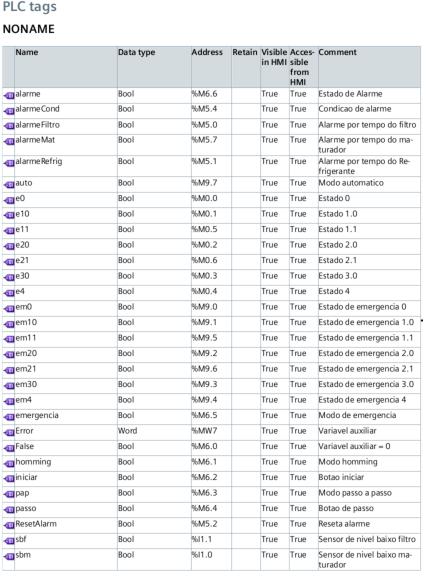
\includepdf[scale=0.6,pages={1},pagecommand=\subsection{Tabela de Variáveis}]{table.pdf}
\label{apx:table}
\includepdf[scale=0.6, pages={2-}]{table.pdf}
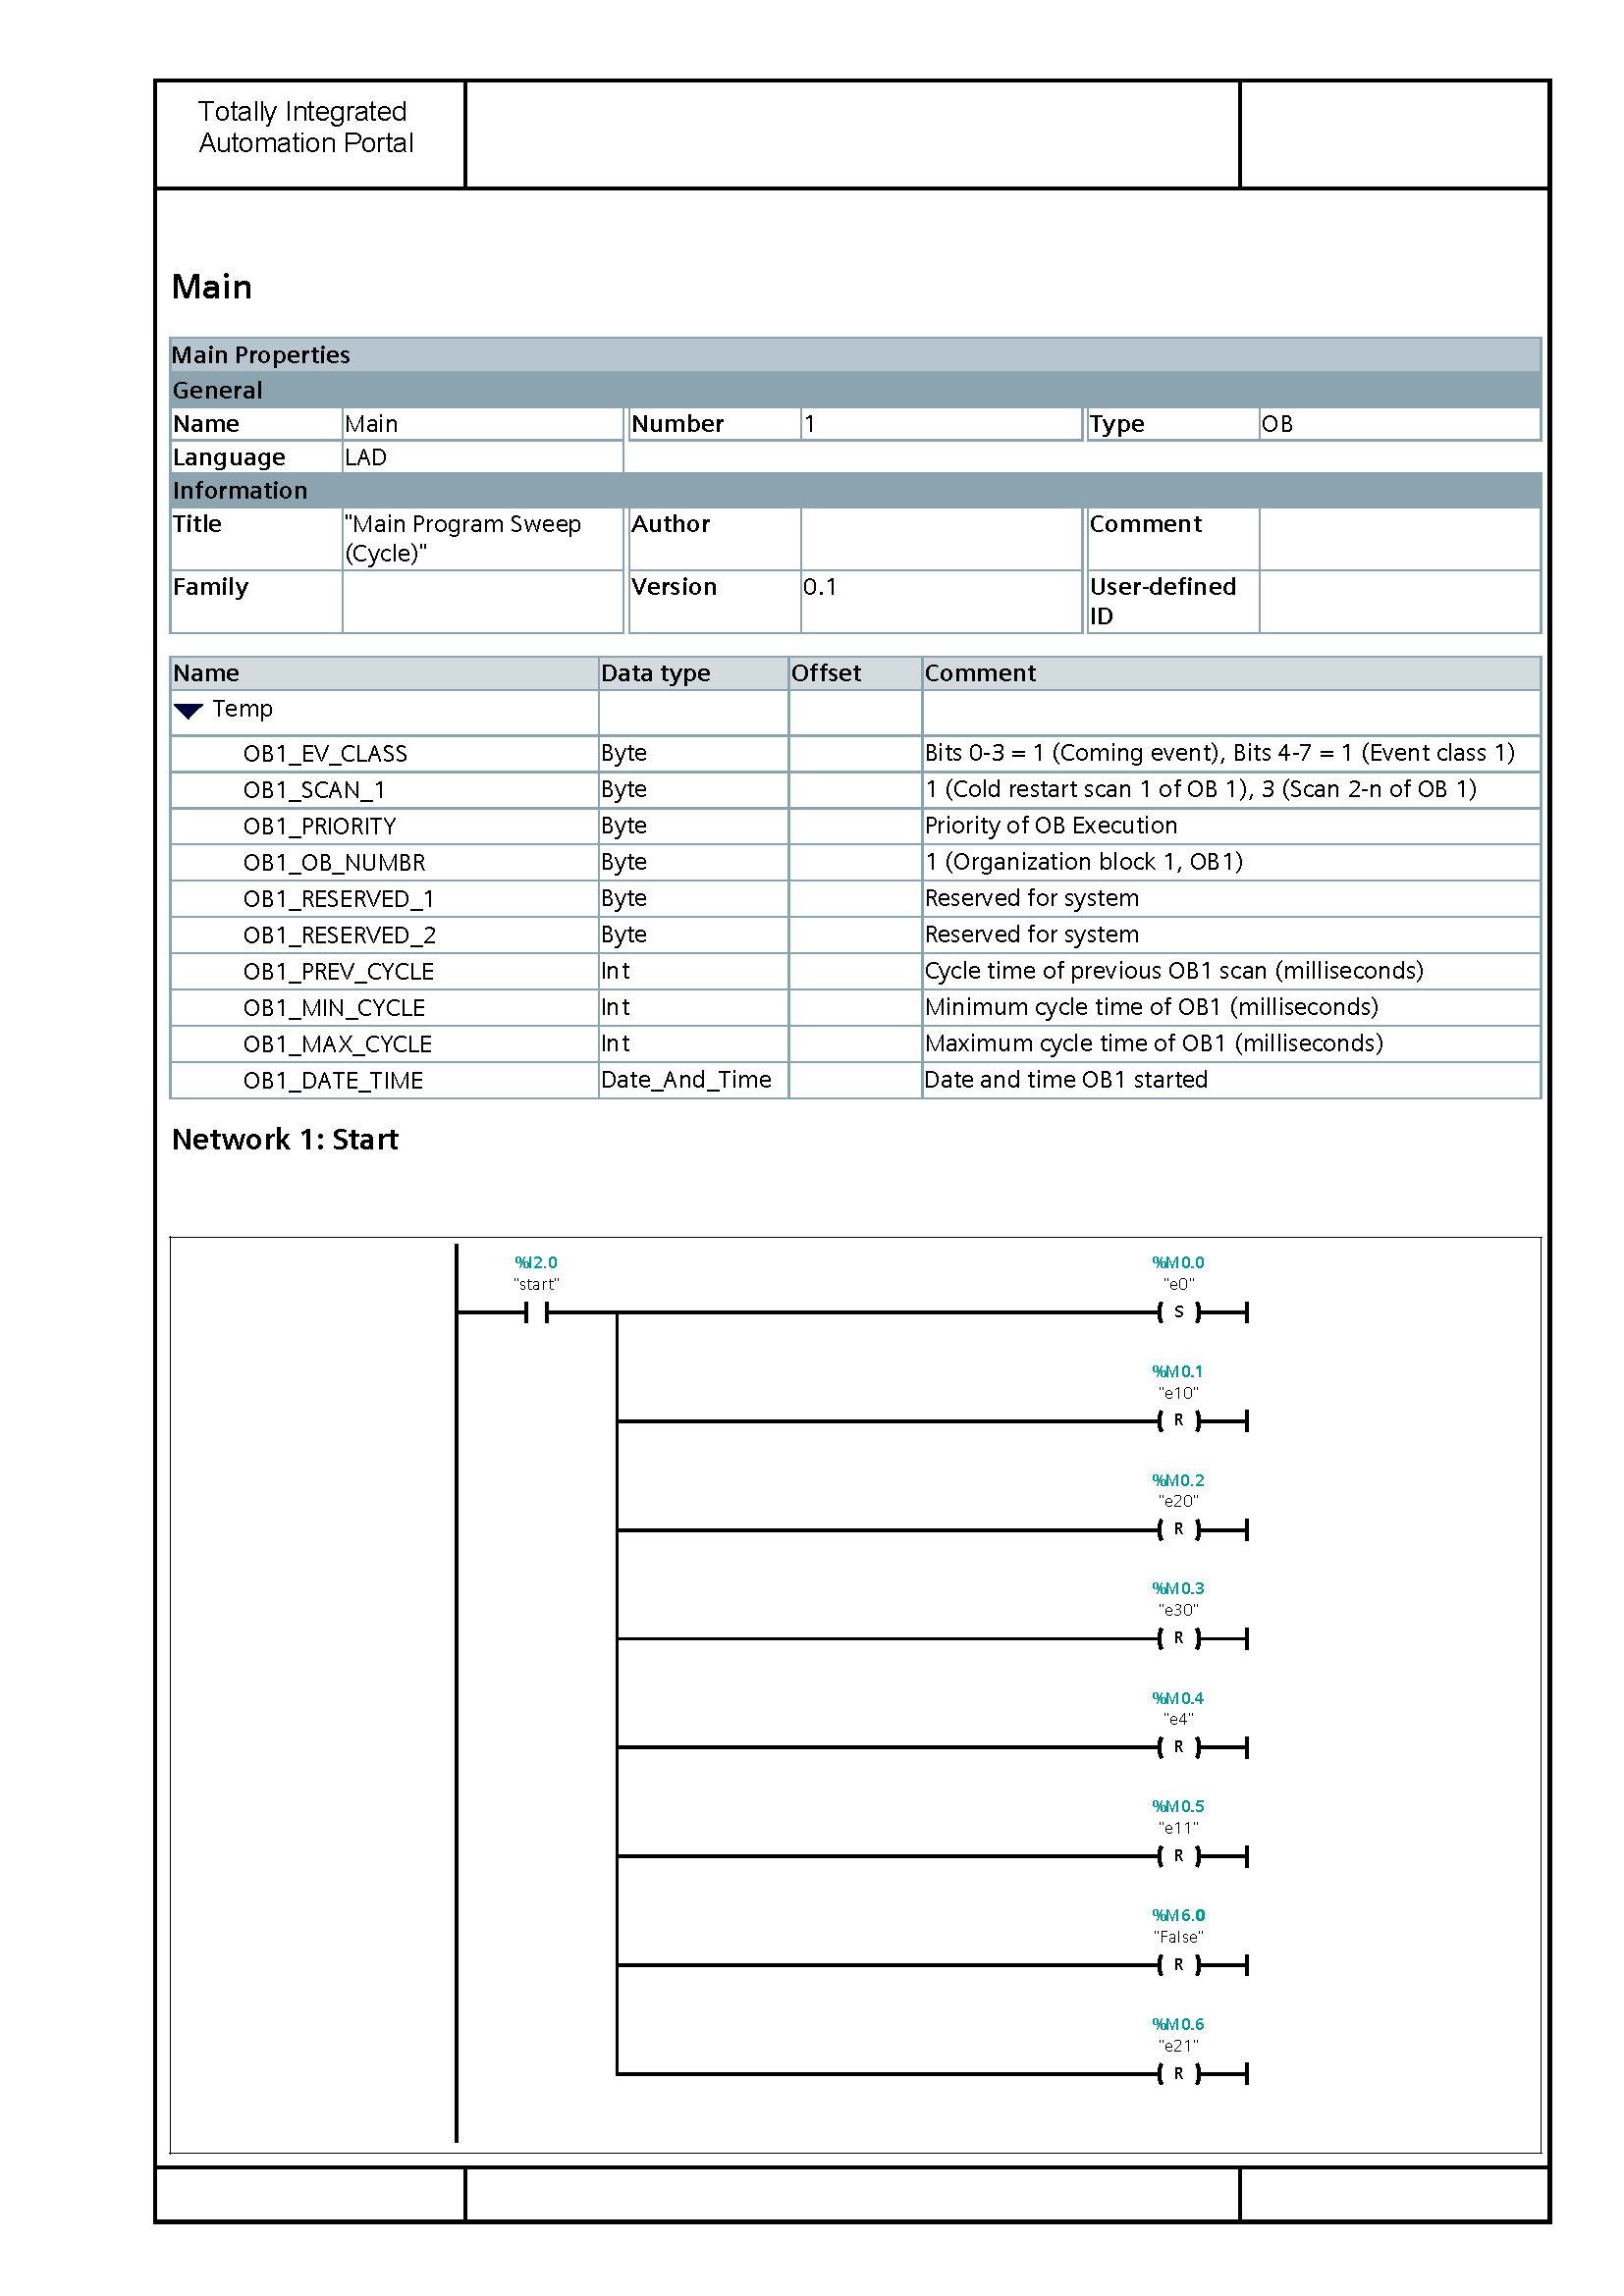
\includepdf[scale=0.6, pages={1}, pagecommand=\subsection{Implementação Ladder}]{ladder.pdf}
\label{apx:ladder}
\includepdf[scale=0.6, pages={2-}]{ladder.pdf}
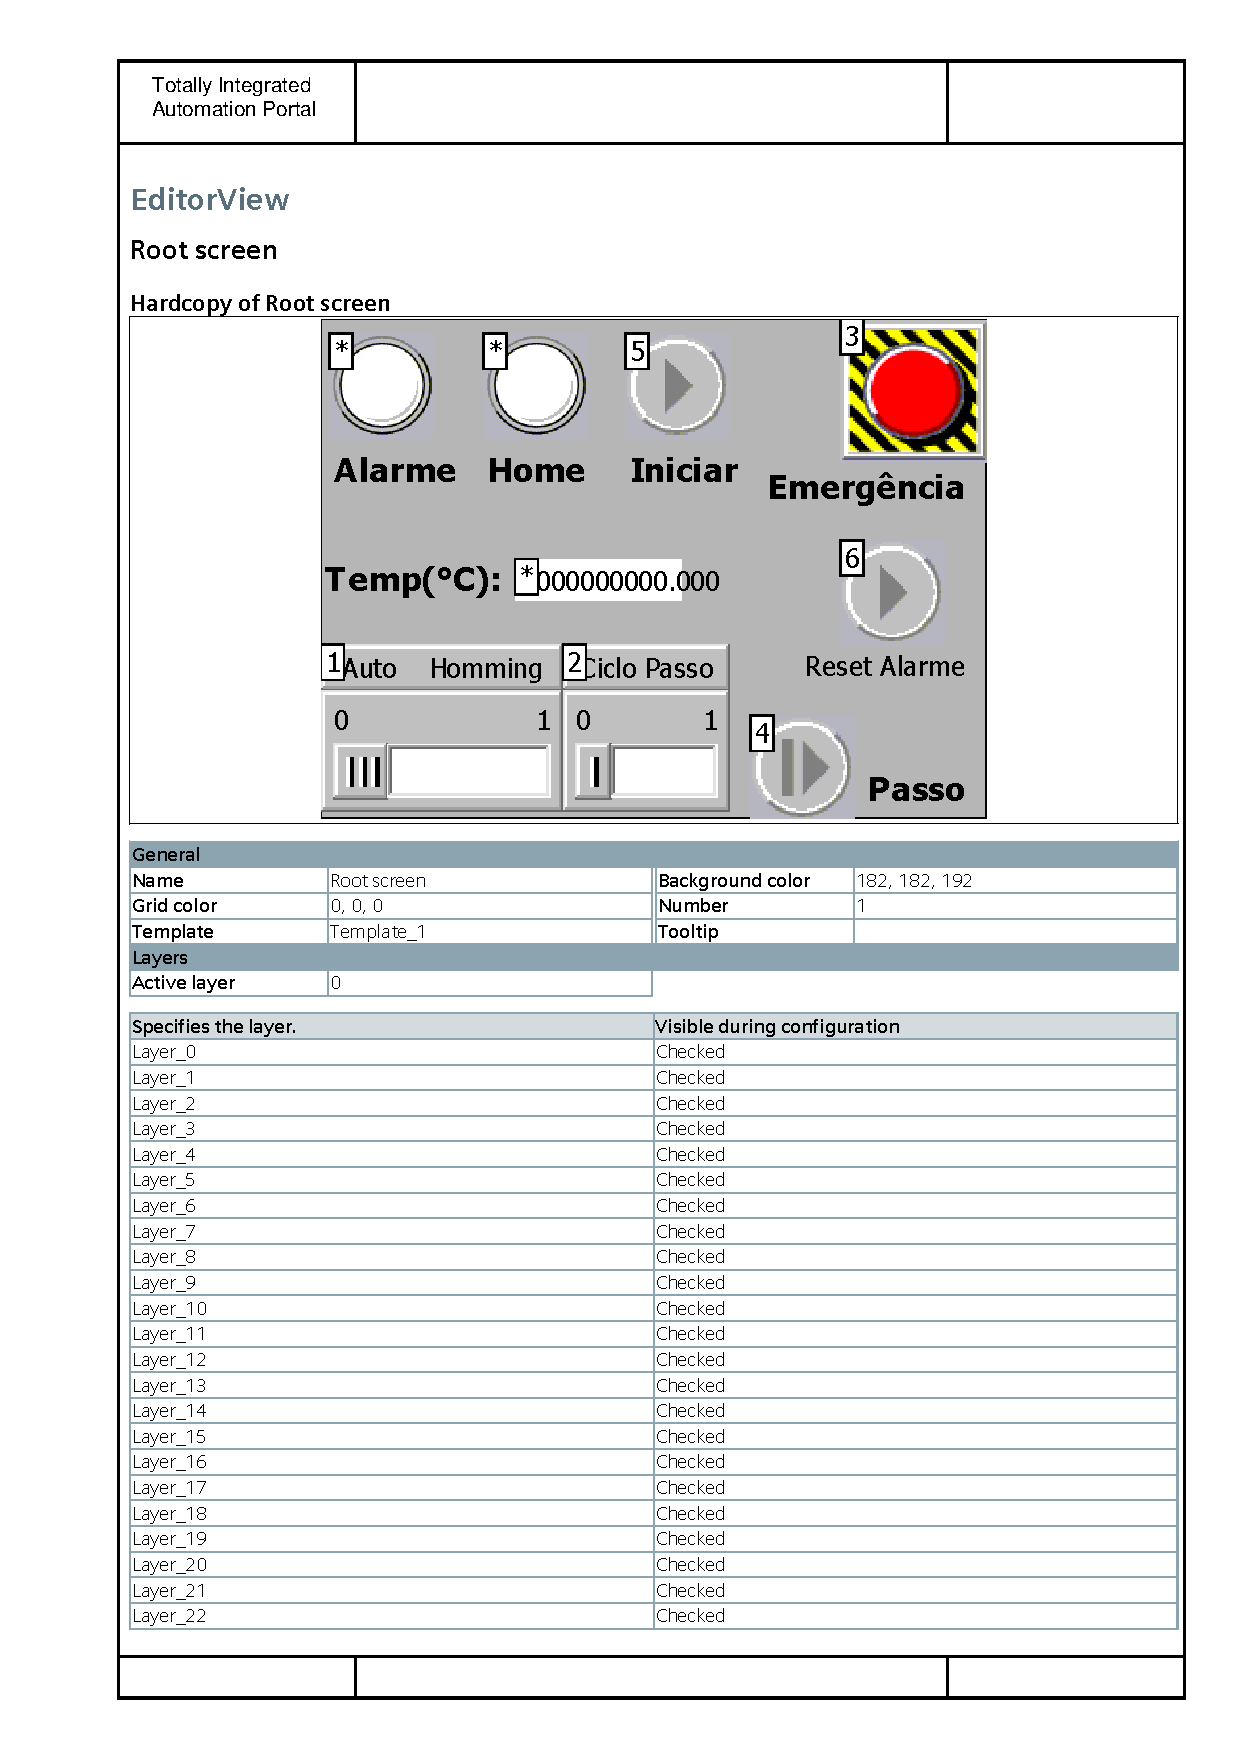
\includepdf[scale=0.68,pages={1},pagecommand=\subsection{Detalhes da IHM}]{ihm.pdf}
\label{apx:ihm}
\includepdf[scale=0.68,pages={2-}]{ihm.pdf}

\twocolumn[{
	\begin{thebibliography}{5}
		% LINK BOM http://www.ufrgs.br/alimentus1/feira/prcerea/cerveja/fluxo.htm
		\bibitem{roteiro4} MASTELARI, N. ``Maturação e Filtração"
	\end{thebibliography}
}]

\end{document}
